\begin{document}

%intro
\subsection{Definition of the Seasons}

\subsection{Method}

\subsection{Results}
%The date is represented by the day of the year (i.e. from 1 to 365 or 366).

\begin{figure}[h!]
\centering
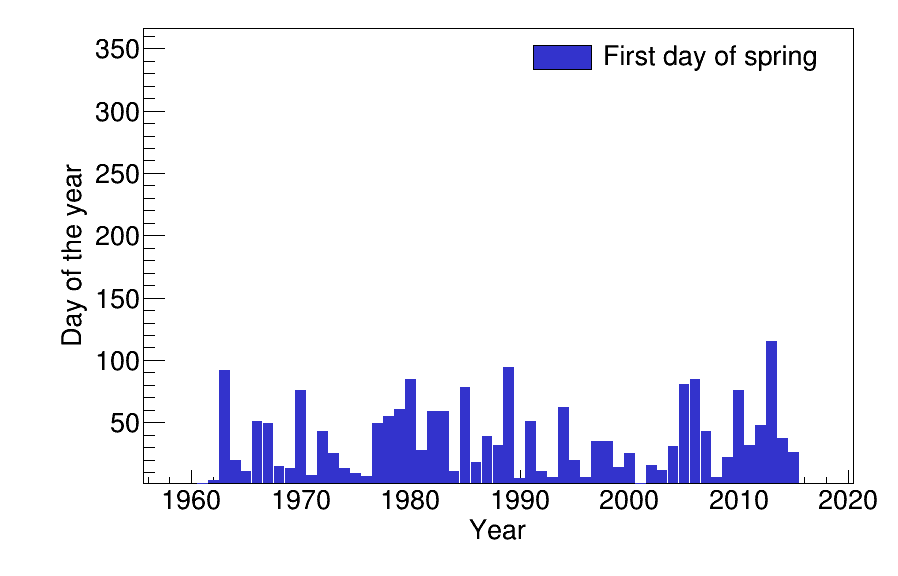
\includegraphics[width=0.85\textwidth]{springStart.png}
\vspace{-10pt}
\caption{The first day on which spring starts for each year in Lund.} 
\label{fig:spring}
\end{figure}

\begin{figure}[h!]
\centering
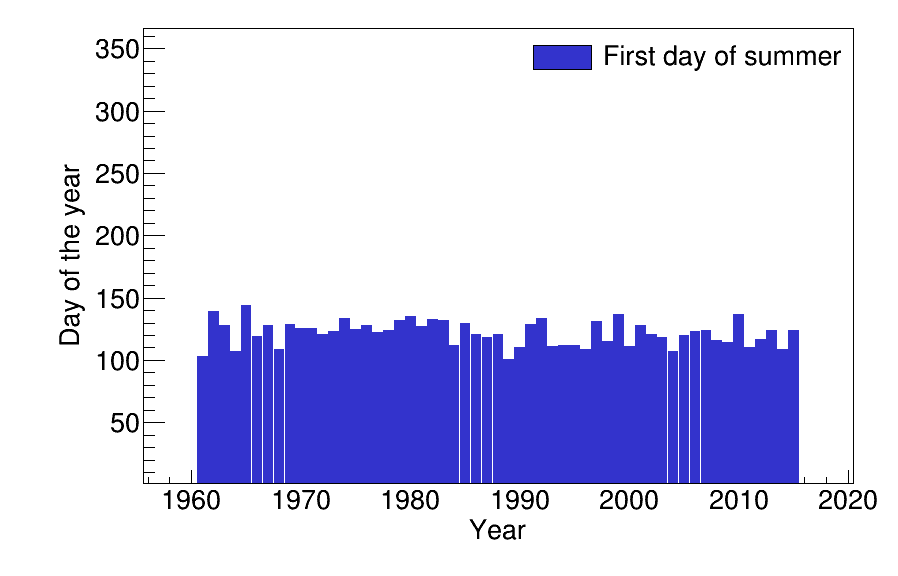
\includegraphics[width=0.85\textwidth]{summerStart.png}
\vspace{-10pt}
\caption{The first day on which summer starts for each year in Lund.} 
\label{fig:summer}
\end{figure}

\begin{figure}[h!]
\centering
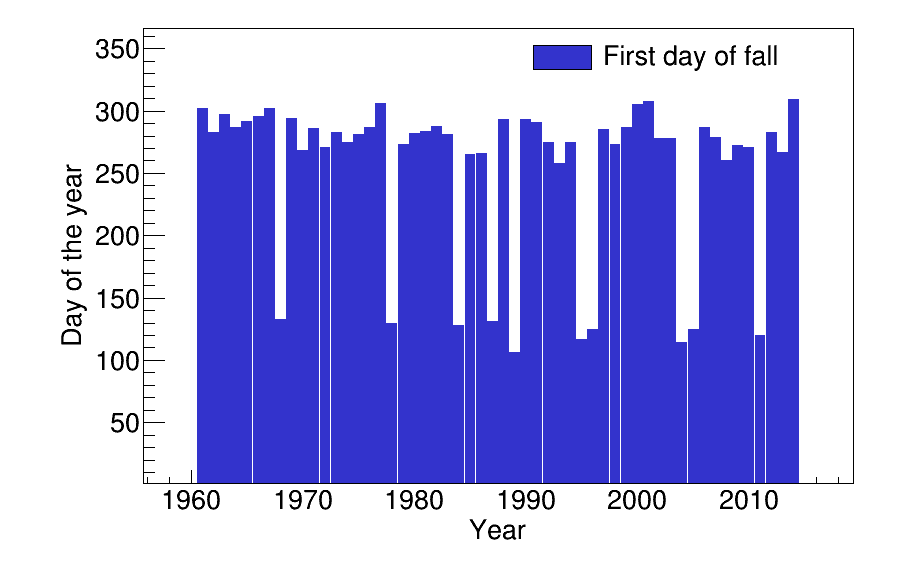
\includegraphics[width=0.85\textwidth]{fallStart.png}
\vspace{-10pt}
\caption{The first day on which fall starts for each year in Lund.} 
\label{fig:fall}
\end{figure}

\begin{figure}[h!]
\centering
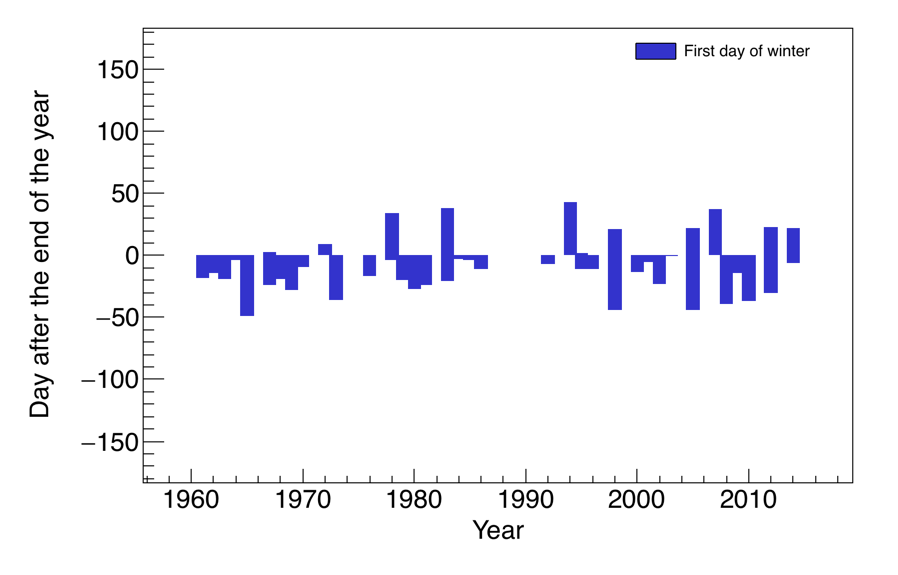
\includegraphics[width=0.85\textwidth]{winterStart.png}
\vspace{-10pt}
\caption{The first day on which winter starts for each year in Lund. The day is given relative to the start of a new year, all negative numbers are before the $1^{\text{st}}$ of January and all the positive numbers are on or after the $1^\text{st}$ of January.}
\label{fig:winter}
\end{figure}

\end{document}
